\chapter{Design}
\label{chap:figtab}
\label{chap}
\section{Overview}

 The requirement is to solve the issue of user interface, data management and control. So we have designed this software with the intention to address this issues. Therefore the design approach comprises the various element that address the issues and provide required solution for creating the specifications. We have designed web interface that provides interaction between user and the system. This idea addresses the issue of user access by proving a dynamic web page where users can simultaneously access the system via the internet rather than performing direct command prompt on the machines. This web page is managed by a client and web server, which serves a channel between the user and the database. We have designed a operation database management system that address the issue of system management. This will take store data from the user interface and also retrieve data to the inventory on the web page via the server. As user log on to the their account on the web page the server will pass this information to the  database which is controlled by the main program (command protocol). The main program is design to initiate and execute the command protocols to the system. It contains all the logic that process the user request and interaction between the system and the machine. Below is a figure that describe the flow of the software design in terms of operational structure.
 
 \begin{figure}[h]
\includegraphics[width = \linewidth]{Design.eps}
\label{fig:Design structure}
\caption{The main software design}
\end{figure}

\section{Web Interface}
The web interface represents the user interface (UI) where users get access to the Clowder system dynamically. It is the main part of the design because it represents the front end of the software.  It contain all the necessary elements required to have dynamic and secure access to the system. The elements includes:
\begin{description}
  \item[$\bullet$] Forms
  \item[$\bullet$] Input controls
  \item[$\bullet$] Navigational component
  \item[$\bullet$] Containers
\end{description}
\section{Forms}
User log in and date entries are the main key to accessing the system. Forms are one the elements that provides the ability to input data to the system.The form is used to submit user details and other data to the database. We have the user login form which takes is used for entering user profile details, and the query forms which is used for submitting data such as machines and reservations details. When data is submitted with HTML form, the server call the html template handler to parse this data to the server to store in the database. This is how the system receive data from the users. For example, when a user create a new profile, we take
\begin{figure}[h]
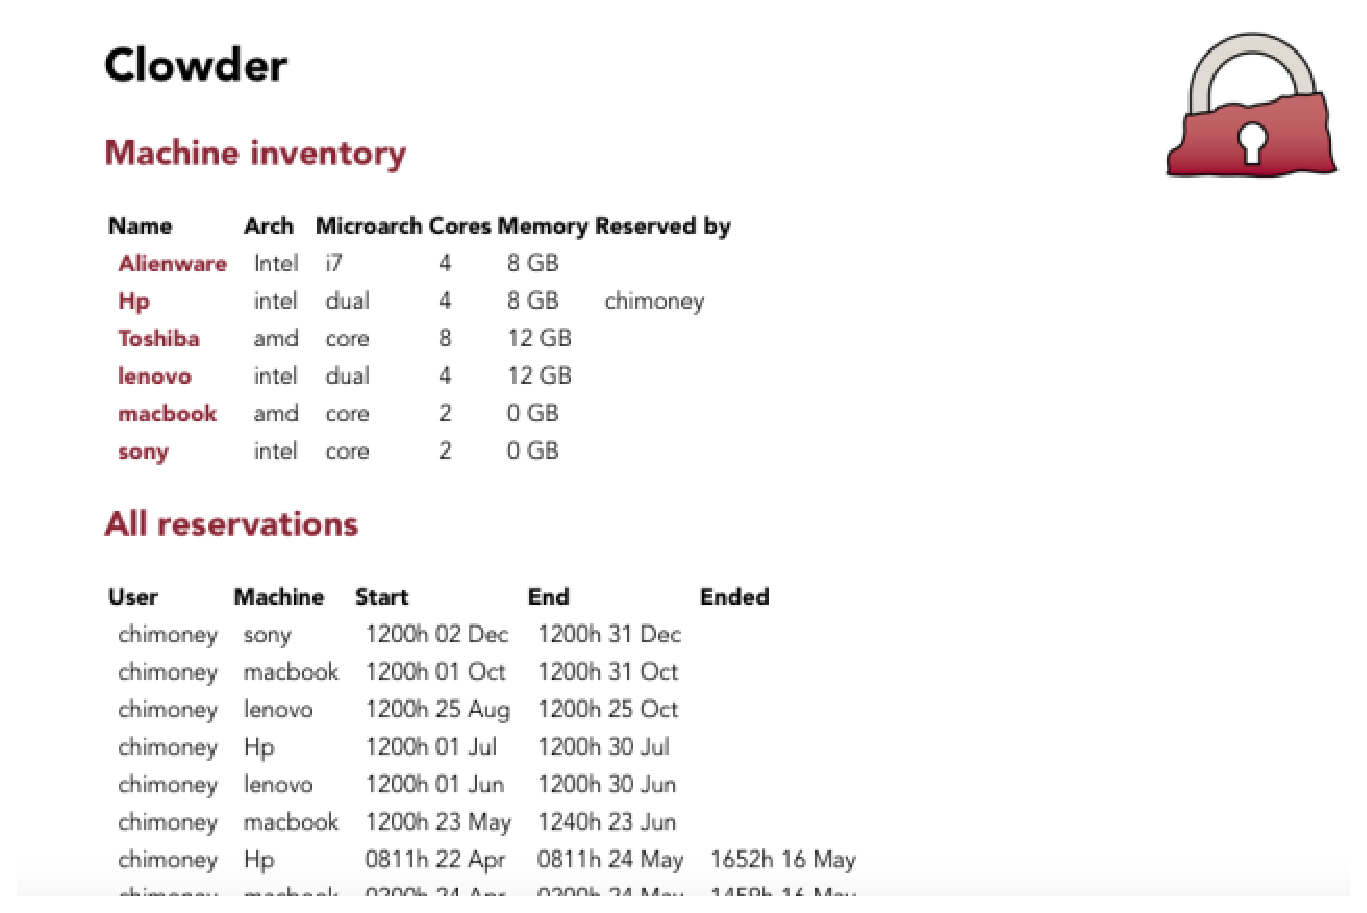
\includegraphics[width = \linewidth]{mainpage.eps}
\label{fig:Web Inteerface}
\caption{The main page of the interface}
\end{figure}

\section{Input Controls}
We design the web interface with some input controls that provide the necessary component that fulfill the specifications. 

\section{Server}
\section{Database}
\section{Program}

